\question 在某页式存储管理系统中,页表内容见表3-10。
若页面的大小为4KB,则地址转换机构将逻辑地址0转换成的物理地址是( ~)。

~
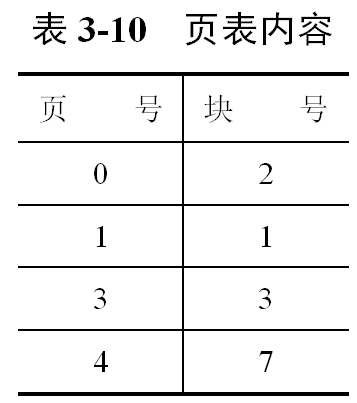
\includegraphics[width=1.15625in,height=1.30208in]{computerassets/A5A380C2BBD77AC406A4715BAE093930.png}
\par\twoch{\textcolor{red}{8192}}{8193}{2048}{2049}
\begin{solution}本题中页的大小为4KB,从表中可知,每个页存储在一个块中,即每个块大小为4KB。逻辑地址0对应的页号为0,表中对应的块号为2。第0块物理地址范围为0~4095;第1块物理地址范围为4096~8191;第2块物理地址范围为8192~12287。本题易错在逻辑地址、物理地址、块号都是从0开始编址的,而不是1。
\end{solution}
\question 请求分页存储管理的主要特点是( )
\par\twoch{消除了内部碎片}{\textcolor{red}{扩充了内存}}{便于动态链接}{便于信息共享}
\begin{solution}请求分页存储管理是为了解决内存容量不足而使用的方法,基于局部性原理实现了以时间换空间的目的。其主要特点自然是从逻辑上扩充了内存。
\end{solution}
\question 在请求分页存储管理中,每个页表的表项实际上是用于实现
\par\twoch{访问内存单元}{静态重定位}{\textcolor{red}{动态重定位}}{装载程序}
\begin{solution}请求分页存储管理的地址重定位方式为动态重定位,这是因为程序的某个页面可能会由于调入调出而在不同时期存储在不同的页框内,因此是动态重定位。页表项所包含的信息就是逻辑地址到物理地址的映射,因此这里页表项的作用就是实现动态重定位。
\end{solution}
\question 作业在执行中发生缺页中断,经操作系统处理后应让其执行( )指令
\par\twoch{被中断的前一条}{\textcolor{red}{被中断的那一条}}{被中断的后一条}{启动时的第一条}
\begin{solution}因为中断是由执行指令自己产生的,而且还没有执行完,故中断返回时应当重新执行被中断的那一条指令。
\end{solution}
\question (四川大学,2002年)请求分页存储管理调度的主要特点是
\par\twoch{消除了页内零头}{\textcolor{red}{扩充了内存}}{便于动态链接}{便于信息共享}
\begin{solution}请求分页存储管理属于虚拟存储管理方式,虚拟存储器解决的就是在逻辑上扩充内存容量的问题。本题可采用排除法,页式存储管理是无法消除内部碎片(即页内零头)的,因此选项A不是。
便于动态链接和便于信息共享都是段式存储管理的特点,因此选项C、D都不是。
\end{solution}
\question 假定有一个请求分页存储管理系统,测得系统各相关设备的利用率为:CPU为10\%,磁盘交换区为99.7\%;其他I/O设备为5\%。试问:下面(
)措施可能改进CPU的利用率? Ⅰ.增大内存的容量 Ⅱ.增大磁盘交换区的容量
Ⅲ.减少多道程序的度数 Ⅳ.增加多道程序的度数 Ⅴ.使用更快速的磁盘交换区
Ⅵ.使用更快速的CPU
\par\twoch{Ⅰ、Ⅱ、Ⅲ、Ⅳ}{\textcolor{red}{Ⅰ、Ⅲ}}{Ⅱ、Ⅲ、Ⅴ}{Ⅱ、Ⅵ}
\begin{solution}本题考查分页存储管理的内容。首先分析题目给出的条件:CPU和I/O设备占用率较低,而磁盘交换区占用率非常高,说明当前系统频繁缺页,频繁进行页面置换,导致真正执行任务的时间变短,效率变低,系统发生抖动。要缓解这种情况,需要降低系统缺页率,才能使系统有更多时间来处理任务而不是置换页面,根据这一思路来分析选项。①Ⅰ正确:增大内存的容量。增大内存可使每个程序得到更多的页面,能减少缺页率,因而减少换入换出过程,可提高CPU的利用率。②Ⅱ错误:增大磁盘交换区的容量。因为系统实际已处于频繁的换入换出过程中,增加磁盘交换区容量也不能降低缺页率,因此增大磁盘交换区的容量无用。③Ⅲ正确:减少多道程序的度数,可以提高CPU的利用率。因为从给定的条件中可知,磁盘交换区的利用率为99.7\%,说明系统现在已经处于频繁的换入换出过程中,可减少主存中的程序,这样每个进程分配到的内存空间会相对增大,可以有效降低缺页率。④Ⅳ错误:增加多道程序的度数。系统处于频繁的换入换出过程中,再增加主存中的用户进程数,只能导致系统的换入换出更频繁,使性能更差。⑤Ⅴ错误:使用更快速的磁盘交换区。因为系统现在处于频繁的换入换出过程中,即使采用更快的磁盘交换区,其换入换出频率也不会改变。⑥Ⅵ错误:使用更快速的CPU。系统处于频繁的换入换出过程中,CPU处于空闲状态,利用率不高,提高CPU的速度无济于事。综上分析,Ⅰ、Ⅲ可以改进CPU的利用率。
\end{solution}
\question 在请求分页系统中,没有优先考虑最近使用过的页面的置换算法是
\par\twoch{\textcolor{red}{最佳置换算法}}{最近最久未使用算法}{先进先出算法}{时钟置换算法}
\begin{solution}最佳置换算法采用``向后看''的思想,没有优先考虑最近使用过的页面。
\end{solution}
\question 考虑页面替换算法,系统有m个页帧(Frame)供调度,初始时全空;引用串(Reference
String)长度为p,包含了n个不同的页号,无论用什么算法,缺页次数不会少于
\par\twoch{m}{p}{\textcolor{red}{n}}{min(m,n)}
\begin{solution}本题考查的知识点是页面置换算法,但考查的角度较为灵活,并非考查页面置换算法的使用,而是讨论置换算法的缺页次数的界限,需要考生深入理解导致页面置换的原因后才能答对。引用串的长度为p,那么即使每次有页面请求都发生缺页,缺页的次数也是p,所以p是缺页次数的上限。不同的页号数为n,那么至少每种页号第一次出现的时候内存中不会有这种页号存在,所以每种页号第一次出现的时候必然发生缺页,所以缺页次数的下限是n。故答案选C。
\end{solution}
\question 假定一个分页虚拟存储系统的虚拟地址为40位,物理地址为36位,页大小为16KB,按字节编址。若页表中有有效位、存储保护位、修改位、使用位共占4位,磁盘地址不在页表中,则该存储系统中每个进程的页表大小为
\par\twoch{1MB}{16MB}{\textcolor{red}{256MB}}{1G}
\begin{solution}C。 页表大小 = 页表项大小×页数。那么求得页表项大小和页数即可得到答案。
该虚拟存储系统最大寻址空间为2\^{}40,又按字节寻址,那么总容量即为2\^{}40B。又页大小为16KB,所以虚拟页数为2\^{}40B/16KB=2\^{}26页。又物理页面和虚拟页面大小相等,所以物理页数为2\^{}36B/16KB
=2\^{}22页,即物理页号为22位。每个页表项包括有效位、存储保护位、修改位、使用位和物理页号,所以其位数为4+22=26。又最小寻址单元为1B,为了简化对页表项的访问,每个页表项取32位,即4B。
综上,页表项大小为4B,页数为2\^{}26。则页表大小=4B×2\^{}26=256MB。
\end{solution}
\question 在缺页处理过程中,操作系统执行的操作可能是( )。 Ⅰ.修改页表 Ⅱ.磁盘I/O
Ⅲ.分配页框
\par\twoch{仅Ⅰ、Ⅱ}{仅Ⅱ}{仅Ⅲ}{\textcolor{red}{Ⅰ、Ⅱ和Ⅲ}}
\begin{solution}在进程刚启动时,所有页面都未调入内存,此时产生缺页中断,发现所缺页面不在内存(并不存在于页表中,也没有对应的页框号),产生磁盘I/O,将页面从外存调入内存中,并为这个页面分配一个空闲页框,修改页表相关信息。因此所有情况都发生了,答案选择D。
【总结】
复习调用页面的流程:在存在快表的系统中,首先查找快表,如果快表命中,则直接产生物理地址并访问;如果快表未命中,则查找页表,页表中存在对应页,则生成物理地址并访问;如果页表中不存在,则说明尚未调入内存,产生缺页中断并按照上面所说的流程将页调入并修改相关数据结构。由此可知,题目中的3种情况只有在缺页时发生,而且必然同时发生。
\end{solution}
\question 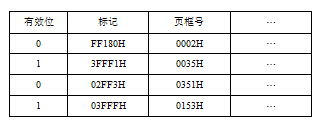
\includegraphics[width=3.36458in,height=1.26042in]{computerassets/44e3f2881e7837913afca6cad4646bcb.jpeg}~

某计算机主存地址空间大小为256MB,按字节编址。虚拟地址空间大小为4GB,采用页式存储管理,页面大小为4KB,TLB(快表)采用全相联映射,有4个页表项,内容如上表所示。则对虚拟地址03FF
F180H进行虚实地址变换的结果是( ~)
\par\fourch{\textcolor{red}{015 3180H}}{003 5180H}{TLB缺失}{缺页}
\begin{solution}由于页面大小为4KB,所以页内地址为12位。于是可以得到虚拟地址03FF
F180H的页内地址为180H,故页号为03FFFH。由表10-8可知,页标记为03FFFH所对应的页框号为0153H,于是将页框号与页内地址进行拼接,即可以得到虚实地址变换的结果是015
3180H。
\end{solution}
\question 若用户进程访问内存时产生缺页,则下列选项中,操作系统可能执行的操作是(
)。 Ⅰ.处理越界错 Ⅱ.置换页 Ⅲ.分配内存
\par\twoch{仅Ⅰ、Ⅱ}{\textcolor{red}{仅Ⅱ、Ⅲ}}{仅Ⅰ、Ⅲ}{Ⅰ、Ⅱ和Ⅲ}
\begin{solution}用户进程访问内存时缺页会发生缺页中断。发生缺页中断,系统执行的操作可能是置换页面或分配内存。系统内没有越界的错误,不会进行越界出错处理。
\end{solution}
